\section{Design}
\label{system_design}
Based on the design goals presented in Section \ref{goals}, we have designed 
and developed a system, \system{}, that allows users to route around a specified 
country.

\subsection{Architecture}

There are three main components to \system{}: the oracle, the relays, and the 
clients.  Figure \ref{fig:arch} shows how the system components
interact to allow a client to access web content while simultaneously avoiding 
a given country.  We employ the most effective country avoidance technique that 
we found in Section \ref{avoid_results}, an overlay network.  The overlay network 
consists of a set of relays, which run as proxy servers.  \system{} also uses 
the same measurement methods used in previous sections for characterizing routing 
detours.  These measurement methods are used learn the paths between clients, 
relays, and domains, and they are stored at the oracle.  The oracle uses the 
measured paths to decide that relay R should be used when a client in location L 
is accessing domain D and wants to avoid country C.  These decisions are made 
for many R, L, D, and C combinations, and also stored at the oracle.  A 
client can access these decisions to route around a country that they wish 
to avoid.

\begin{figure}[t]
\centering
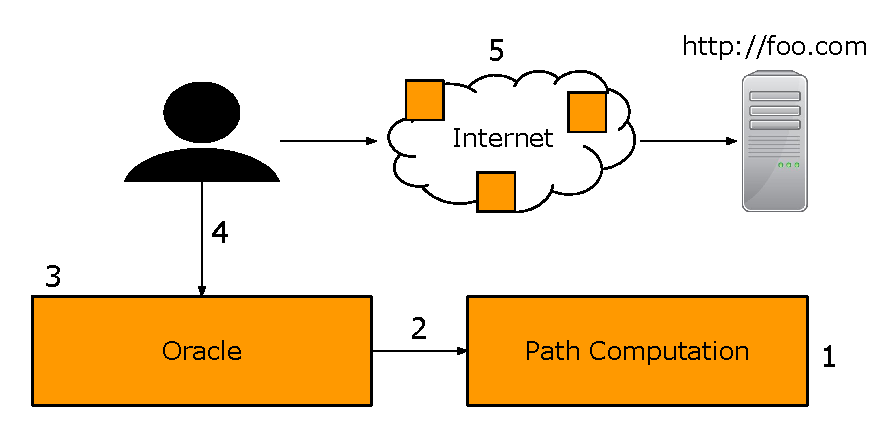
\includegraphics[width=.5\textwidth]{system_arch}
\caption{\system{} architecture. 1) Paths are computed between clients and relays, 
relays and domains, relays and clients, and clients and domains.  2) The oracle 
aggregates all paths.  3)  The oracle generates a PAC file that specifies which 
domains should be accessed through which relays (based on the measured paths).  
4) The client configures her browser to use the oracle-generated PAC file.  5) 
The client's traffic is routed through relays (or direct paths) to access domains, 
while avoiding a client-specified country.}
\label{fig:arch}
\end{figure}

\subsection{Systematic Path Measurement}
As mentioned earlier, \system{} is an overlay network that is measurement-driven.  
The system includes a set of relays that function as TCP proxy servers.  The system 
was designed for accessing web content seamlessly through the overlay network, and 
TCP proxies support this.  IP layer proxies force the client to download and 
install software, which makes the system less user-friendly.  Therefore, we 
chose to use TCP proxies instead of some other type of proxy, such as IP layer proxies.  
Once we established the TCP proxies, or relays, the system needed a way to 
learn which proxy to use when accessing a given domain.  Here we explain which paths we measure, 
how and where they are measured, as well as the challenges associated with the 
role of measurement in the system.  

All of the paths are measured using {\tt 
traceroute}, which is then mapped to the country level using the same methods as 
described in Section \ref{datasets} and shown in Figure 
\ref{fig:analysis_pipeline}.  The paths we measure are the: forward paths from 
the client to each relay, forward paths from each relay to each domain, forward 
paths from the client to each domain, and reverse paths from each relay to the 
client. Figure \ref{fig:path_components} shows the forward and reverse paths when accessing 
content using relays; path component 3) is the only path we cannot measure because we have no 
vantage point at or near the domain from which to run {\tt traceroute}.

{\bf Client to Relay Paths.} As previously mentioned, one of the goals of the 
system is usability, and therefore, the client should not have to download software 
or perform any measurements.  Therefore, 
the paths from clients to relays are measured using RIPE Atlas probes.  A probe 
is selected from a geographically close location to the client (i.e., the same 
country), and the oracle triggers the probe to run {\tt traceroute} measurements 
to each relay in the system.  After collecting the responses, the oracle maps 
the IP-level paths to country-level paths and stores the results.

{\bf Relay to Client Paths.} The relays are set up with software to run 
{\tt traceroute} measurements to the IP addresses of RIPE Atlas probes, which 
represent clients.  They then map the responses to country-level paths, and 
store them locally; the oracle will fetch these paths from each relay. 

{\bf Relay to Server Paths.} The software on the relays also runs {\tt 
traceroute} measurements to each domain.  Similar to the paths to clients, these 
are mapped to country-level paths, stored, and then fetched by the oracle.

{\bf Client to Server Paths.} In the case that a path from a client to a 
domain does not pass through the country specified to avoid {\it by default}, 
then none of the proxies should be used.  If a proxy is used, then it may 
actually be causing the path to traverse more countries (unnecessarily).  These 
paths are measured using the RIPE Atlas probes in similar locations as the 
clients, and the oracle triggers {\tt traceroute} measurements to be run from 
them to each of the domains.  The results are converted to country-level paths 
and stored on the oracle.  

Each of these types of paths must be computed initially, but also re-computed 
as paths may change.  To our knowledge, there has not been any previous work 
on how often country-level paths change; prior work has explored how often 
AS-level paths change.  To measure how often country-level paths change, we 
computed the paths from relays to domains once every two hours and once every 
hour.  On average, the path to X domains changed every two hours, and the path 
to Y domains changed every one hour.  As it takes approximately 30 minutes to 
compute all paths, \system{} re-computes the paths every one hour to incorporate 
the most recent country-level paths in the system.

\begin{figure}[t]
\centering
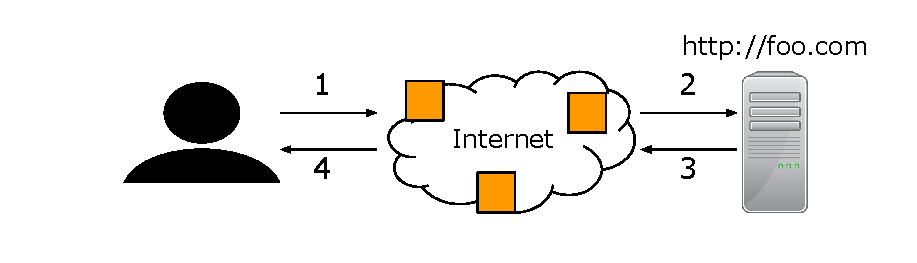
\includegraphics[width=.5\textwidth]{four_paths}
\caption{The path of a web request through a \system{} relay, to the domain, and back. 
1) forward path from client to relay; 2) forward path from relay to domain; 3) reverse 
path from domain to relay; 4) reverse path from relay to client.  \system{} measures 
all paths except for path 3) due to a lack of vantage points at domain locations.}
\label{fig:path_components}
\end{figure}

As seen in Figure \ref{fig:path_components}, there are four path components 
when a client accesses web content through \system{}.  The system measures three 
out of the four paths; the reverse path from the domains (servers) to the relays 
is challenging to measure due to a lack of vantage points.  Despite not 
calculating all of the country-level path components, we can show that the 
country a client is attempting to avoid cannot conduct traffic analysis attacks 
on the traffic because {\it at most} the attacker is only on the reverse path 
from the server to the relay.  An attacker would need at least two path 
components to perform traffic analysis. 

\subsection{Automated Relay Multiplexing}
\label{multiplex}
After measuring and aggregating the country-level paths, the oracle decides 
which relay to use when accessing specific domains from a specific client 
location.  This decision follows three sequential steps:

\begin{enumerate}
\item If the default path from the client to the domain does not pass through 
the specified country, then do not use any of the relays. Otherwise, continue 
to the next step.
\item For all the paths from the client to the relays, select usable relays 
such that the path does not contain the specified country.
\item From the set of usable relays, if there is a path from a 
usable relay to the domain that does not include the specified country, then 
use that relay for that domain.
\item If there is no path from the client through any of the relays to the domain 
that does not pass through the specified country, then select the relay 
that provides the most avoidance (measured by how many other domains it has 
a path to that avoid the specified country).
\end{enumerate}

The oracle applies this decision process to each domain, and generates a PAC 
file, which specifies which domains should be accessed through which proxy.  A 
sample PAC file is shown in Listing \ref{lst:pac}; in this example, proxy 
1.2.3.4:3128 should be used when accessing {\tt www.google.com}, but proxy 
5.6.7.8:3128 should be used when accessing {\tt www.twitter.com}.  Once the PAC 
file is generated based on the decision chain above, it is published to a URL 
of the format $<$client\_country$>$\_$<$country\_to\_avoid$>$\_pac.pac.  The client 
simply uses this URL to specify their proxy configuration.  As paths are re-computed 
every hour, the PAC file is also re-computed and published every hour.  The PAC files 
are published online, which allows a client to simply configure her settings to 
point at the URL that contains the PAC file.  Whenever the client re-opens her 
browser, the latest PAC file will be used for relay multiplexing.

\subsection{Scaling the System}
\system{} is 
designed in a modular way, and therefore, adding relays is quick, easy, and 
simple.  To add a relay, the system operator must set up a machine as a proxy 
server, install the \system{} relay software, and update the oracle's list of 
relays.  From that point forward, paths will be computed to and from the new 
relay, and clients will be using it as a proxy.  

Adding an oracle is a matter of installing the oracle software on 
a different machine, and specifying the client locations handled by that oracle 
(for example, oracle 1 handles all clients in North America and Europe, and 
oracle 2 handles all clients elsewhere).  Both oracles will publish the PAC files 
to the same server, which causes no changes for the client.

\subsection{Fault Tolerance}
\system{} is resilient to crashed system components, such as a crashed relay or 
oracle.  

{\bf Failed Relay.} If a relay becomes unresponsive, this issue is handled by 
the PAC file.  The PAC file allows the oracle to specify multiple proxies in 
a sequential order, such that if the the first proxy fails, then the second 
proxy is used (and so on).  This feature can be used to specify all of the 
relays that have a path to the domain.  And future work can include relay 
replicas that can be used in the case that a relay crashes.

{\bf Failed Oracle.} A failed oracle can be detected by PAC files that are 
older than 1 hour.  Detecting a failed oracle could trigger a backup oracle 
to re-compute the PAC files periodically.  This is a simple solution because 
the oracles do not need to convey any information among each other, and therefore, 
no information is lost.  We leave the implementation of backup oracles as future 
work.

It is worth noting that without backup oracles, clients can still use the system 
when the oracle fails.  The clients will simply be using stale paths, which are 
likely to be the same original paths, but not always.  


